\documentclass[a4paper,11pt,oneside]{book}

\usepackage[english]{babel}
\usepackage[showframe=false]{geometry}
\usepackage[usenames,dvipsnames]{xcolor}
\usepackage[utf8]{inputenc}
\usepackage[T1]{fontenc}
\usepackage{changepage}
\usepackage[]{algorithm2e}
\usepackage{amssymb}
\usepackage{amsmath}
\usepackage{graphicx}
\usepackage{listings}
\usepackage{verbatimbox}
\usepackage{ulem}
\usepackage{fancyvrb}
\usepackage{float}
\usepackage{hyperref}
\usepackage[parfill]{parskip}
\usepackage{tikz}
\usepackage{pdflscape}
\usepackage{minted}
\usepackage{titlesec}
\usepackage{titleps}
\usepackage{lastpage}
\usepackage{fancyhdr}
\usepackage{etoolbox}
%Following overwrites the page style for chapters
\patchcmd{\chapter}{\thispagestyle{plain}}{\thispagestyle{ruledChapter}}{}{}

%New page style for chapters
\newpagestyle{ruledChapter}{
	\setfoot{}{\thepage\ of \pageref{LastPage}}{}
	\footrule
	\renewcommand\makefootrule{\color{black}\rule[\baselineskip]{\linewidth}{0.4pt}}
}
%New page style for rest
\newpagestyle{ruled}{
	\sethead{\raggedright \chaptername\ \thechapter :\ \chaptertitle}{}{}
	\headrule
	\setfoot{}{\thepage\ of \pageref{LastPage}}{}
	\footrule
	\renewcommand\makeheadrule{\color{black}\rule[-.3\baselineskip]{\linewidth}{0.4pt}}
	\renewcommand\makefootrule{\color{black}\rule[\baselineskip]{\linewidth}{0.4pt}}
}

\expandafter\def\csname PY@tok@err\endcsname{}
\newcommand{\HRule}{\rule{\linewidth}{0.5mm}}
\newcommand{\specialcell}[2][c]{%
  \begin{tabular}[#1]{@{}c@{}}#2\end{tabular}}

\addtocontents{toc}{\protect\thispagestyle{empty}}

\title{}
\author{}
\date{} 

\begin{document}
\begin{titlepage}
\begin{center}

%-----------------------------------------------------------------
%							FRONTPAGE
%-----------------------------------------------------------------
\thispagestyle{empty}

\includegraphics[width=0.55\textwidth]{logo.pdf}\\[1cm]    
\textsc{\Large DM818 Assignment 1}\\[0.5cm]

% Title
\begin{Huge}
\textbf{Matrix Multiplication}
\end{Huge}

\vspace{4cm}

% Author and supervisor
\begin{minipage}{1\textwidth}
\begin{center}
\emph{}\\

Dan \textsc{Sebastian Thrane}\\
\verb!<dathr12@student.sdu.dk>!\\

Lars \textsc{Thomasen}\\
\verb!<latho12@student.sdu.dk>!\\

\end{center}
\end{minipage}
\begin{minipage}{0.4\textwidth}
\end{minipage}

\vfill
\begin{tabular}{ll}
    Aligned SSE: yes \\
    Unaligned SSE: no \\
\end{tabular}
\vfill

% Bottom of the page
{\large Fall 2015}\\

\end{center}
\end{titlepage}

%-----------------------------------------------------------------
%							   TOC
%-----------------------------------------------------------------
\renewcommand{\contentsname}{Table of Contents}
\tableofcontents
\thispagestyle{empty}

%-----------------------------------------------------------------
%						  ACTUAL REPORT
%-----------------------------------------------------------------
\pagestyle{ruled}
\chapter{Introduction}
\setcounter{section}{1}

This report covers the task of optimizing matrix multiplication on a single
core. For this task access to the NERSC cluster has been supplied, thus majority
of the performance tweaking was been focused for this. Code for running on the
SDU Imada terminal room has also been developed, however values are not tweaked
as well there.

\section{Work Load}

This assignment has been done in a group of two, following pair programming
principles. Thus the work load has been evenly divided, majority of the work
load being converting theoretical theories into actual code and doing things
correctly.

\chapter{Optimizations}
% The optimizations used or attempted
% The results of those optimizations
\section{Overview}

The basis of our algorithm is a blocked approach based on a proposed algorithm
from Goto. % TODO Proper reference 

The overall plan for this algorithm consists of three phases:

% TODO Make sure that the following claims are correct. This section is meant to
% be a somewhat informal overview of the algorithm.

\begin{enumerate}
  \item Split the input matrices into slivers. Matrix A will be split into 
  slivers of columns, matrix B will be split into slivers of rows. A is split
  into slivers of columns, and B into rows, because of the access pattern that
  will be used during the actual multiplication phase, and as such improve the
  data access pattern, and minimize the number of movements between memory
  layers.
  \item Split the matrices up into smaller blocks, and begin packing the data.
  The smaller blocks are chosen such that they may reside inside of a single
  memory layer. The data is packed such that it will be placed sequentially in
  memory with accordance to how the data will be accessed by the program. 
  The data should be packed shortly before use, such that it can stay as close 
  to the CPU as possible.
  \item Perform efficient matrix multiplication between these small blocks.
\end{enumerate}

% TODO Talk about sizes of matrices
% Covered in block size part.

The following sections will go into details of how these phases were
implemented, and how the results observed guided further optimizations.

\subsection{Efficient Inner Matrix Multiplication}

It is the job of the other phases to ensure that data is laid out in memory,
such that movement between memory layers are minimized. It is the job of this
phase to as efficiently as possible do raw number crunching.

The Intel architecture available on both Hopper, and on the IMADA machines used
for development, both provide a set of SSE instructions. These instructions are
SIMD instructions. Single instruction, multiple data (SIMD) is a form of
parallelism with multiple processing elements that perform the same operation on
multiple data simultaneously. This means that we can multiply several numbers
with each other at the same time. 

By using SIMD instructions, we are able to cut the K iterations in half by doing
two iterations at the same time with no additional cost. As a result we saw a
significant performance improvement. 

However to using SSE instructions efficiently requires the data to be properly
aligned at a 16-byte offset.
Since we do not have control of how the input data is stored, this will require 
copying the data, and assure that the data is copied to start at a properly 
aligned address. 

The SSE instructions will always work on two double-precision floating point
numbers. This provides us with an edge-case when the inner loop works on
matrices with dimensions that aren't a multiple of two. This problem became even
more important when loop unrolling was performed to further optimize
performance. We simply dealt with the problem by padding the matrices.

% TODO Do we put any code here?
% Seems irrellevant, we were pretty much given the code in examples.

\subsection{Preparing the Data}

In order to improve data locality, and take advantage of loading SSE
instructions, data had to be re-arranged. This required new auxiliary arrays for
the packed data, aligning it for 16 bytes. Since this data would have to be
loaded regardless, then we won't incur much additional movement between the 
memory layers. % TODO Not trivial, not sure this is enough, what about 
% overhead from writing?
% According to goto, there might be a slight, but non-critical overhead.
% Changed a single word to match this.

We first pack the entire B matrix, and then pack the A matrix in slivers of size
$mc$. The order of this packaging ensures that the relevant $mc$ rows of the A
matrix is always in memory along with most, if not all, of the B matrix too. By
packing slivers of the A matrix we are able to increase the block size in
general and still keep it all in memory.

\subsection{Loop Unrolling}

% TODO: I need to read up a slight bit on exactly how this works, but the gist
% of it is correct. (What is the difference between hardware pipelning and
% software pipelining exactly?).

In order to exploit pipe-lining, loop unrolling has been performed in the inner-
most matrix multiplication. By loop unrolling the actual multiplication of the
elements, the hardware is able to do several loads and multiplications at once,
rather than having to wait for a a single to finish and continuing the loop.

To understand this, the following example will try to explain it. Let's say that
if a single load and multiplication takes N time, then by taking advantage 
of pipe-lining, two iterations unrolled into a single one might only take N+1 time 
in total, by doing some of the other tasks while the first ones are finishing.
Effectively cutting off N-1 time compared to a non-unrolled loop. 

% Insert code example here?
% Tried to cover it with the explanation above.

Loop un-rolling would result in diminishing returns at higher values, and as such
it was assumed that the extent to how much could be pipelined at once was reached.

%Padding:

In order to perform loop unrolling, padding was initially used such that fringe
cases would not cause the program to access data outside of the arrays. This
padding was done by simply putting the value 0 into the additional elements
accessed, as this would not change the correctness of the matrix multiplication.

This padding resulted in performance dips for matrix sizes which did not fit
into a multiplicative of the unrolled size. This behaviour is clearly seen in
the figure below. The explanation for this lies in the added calculations of the
zeroes, along with using an auxiliary array for the result matrix.

The auxiliary array was necessary, as padding the result matrix was infeasible
when writing to values outside its array. This writing to a temp array and
moving only the relevant entries to the result matrix. was the best solution 
we could come up with to avoid over-writing critical data.

\begin{figure}
  \centering
  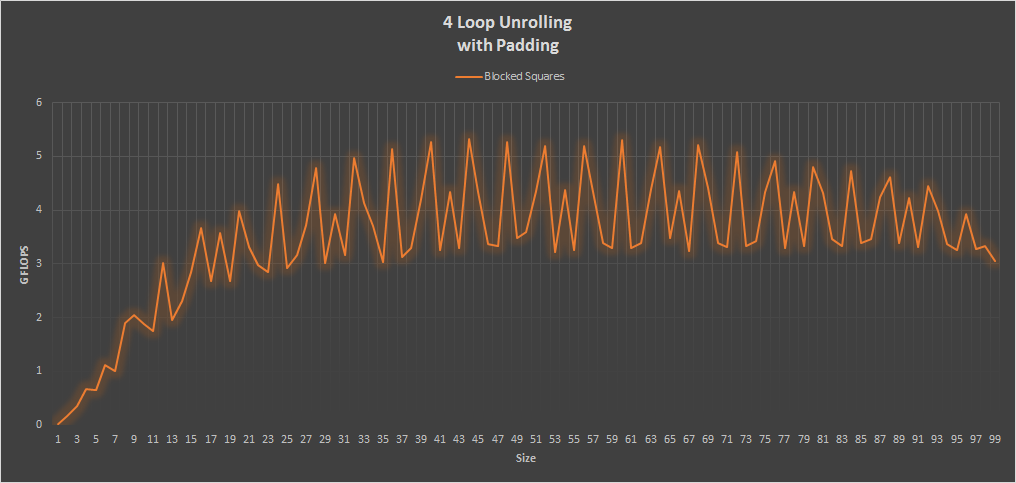
\includegraphics[width=0.9\linewidth]{graph-blocked-padding.png}
  \caption{Example using padding and auxiliary array on every block size. Note 
  this is before this was improved upon.}
  \centering
  \label{fig:sub1}
\end{figure}

This solution was however improved upon by doing an early check of the actual block
size, and then calling the method best fitted for that block size, such that
loop unrolling could be maximized. Thereby avoiding the additional overhead unless
absolutely necessary.

\subsection{Fringe Cases and Padding}

The padding introduced yet another problem. When reaching certain fringe
cases, these padded entries would result in entries into the $C$ matrix which
would be out of bounds.

As we saw in the loop unrolling section, we use different procedures depending
on which case we are dealing with. We used this to avoid adding padding, when we
knew that it wouldn't ever be required. This obviously means that we won't have
to deal with going out of bounds in this special case, since we know that it
cannot happen, due to no padding being added. In the case that padding may be
added, we however had to deal with this problem. The two most simple approaches 
to this are:

\begin{enumerate}
  \item Run-time checks to avoid going out of bounds
  \item Use an auxiliary matrix, which also contains padding, and copy this to 
        the real output matrix
\end{enumerate}

Approach 1 may be the most traditional way of dealing with out-of-bounds
behaviour, when writing code that isn't performance critical. However this
approach leads to a large amount of branching. Which the loop unrolling
optimization also showed, leads to a significant performance loss.

Approach 2 has a small amount of overhead involved in copying the data from the
auxiliary matrix into the output matrix, however our observations showed that
this was still better than going with approach 1.

% TODO Did we ever try using approach 1? Would be nice with some numbers to 
% show that we actually did the right thing
% No we did not, this was assumed. Should really do a quick test of this if
% time allows it.

\subsection{Choosing Block Sizes}
Choosing the best block sizes, such that when packaging the matrices, as much
relevant data as possible would still reside in the biggest cache, thus creating
minimal overhead, is important.

Changing the blocksize will directly affect performance in a positive or negative
direction.
% I really need to do a test of this with a different size, will do later today.

We finally settled on the actual blocksize by testing the algorithm with
slowly increased blocksizes until we would see the performance start to decrease 
rather than increase. While this is not the optimal way, rather than calculating
how much there should be room for, it was our experience that these calculations
did not in fact give the best performance in practice.

\chapter{Performance}

% How the same kernel performs on a different hardware platform (and a small
% discussion of that)

\section{Hopper}
\subsection{Graphs}

% A figure that shows the performance similar than the figure above, but using
% all matrix sizes 2, 3, 4, ..., 769 for a single processor core of NERSC Hopper
% cluster (y-axis should say percentage of peak performace).

Below is a graph comparing the different algorithms. The Naive, Transposed, and BLAS algorithms are the ones from the assignment. The Blocked algorithm is the implementation following the previous sections. All have been run on hopper, scheduled with a single node.

\begin{figure}[H]
  \centering
  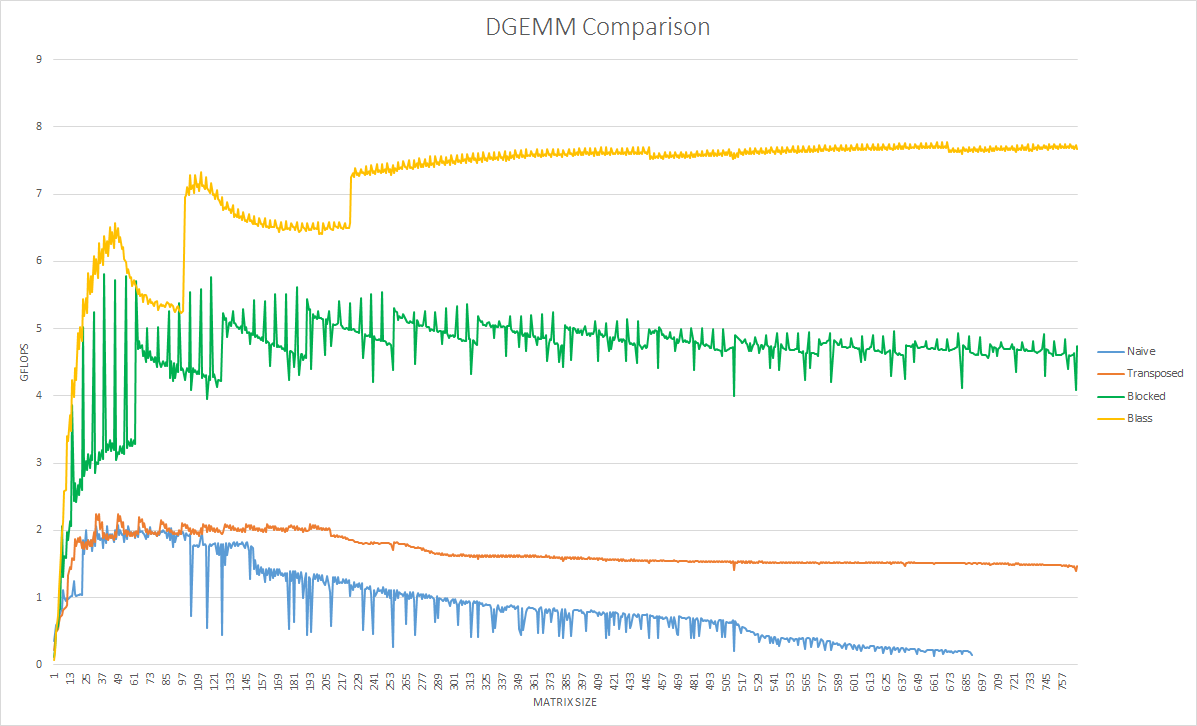
\includegraphics[width=0.9\linewidth]{comparison-graph.png}
  \caption{Comparing different algorithms in GFLOPS.}
  \centering
  \label{fig:sub1}
\end{figure}
\begin{figure}[H]
  \centering
  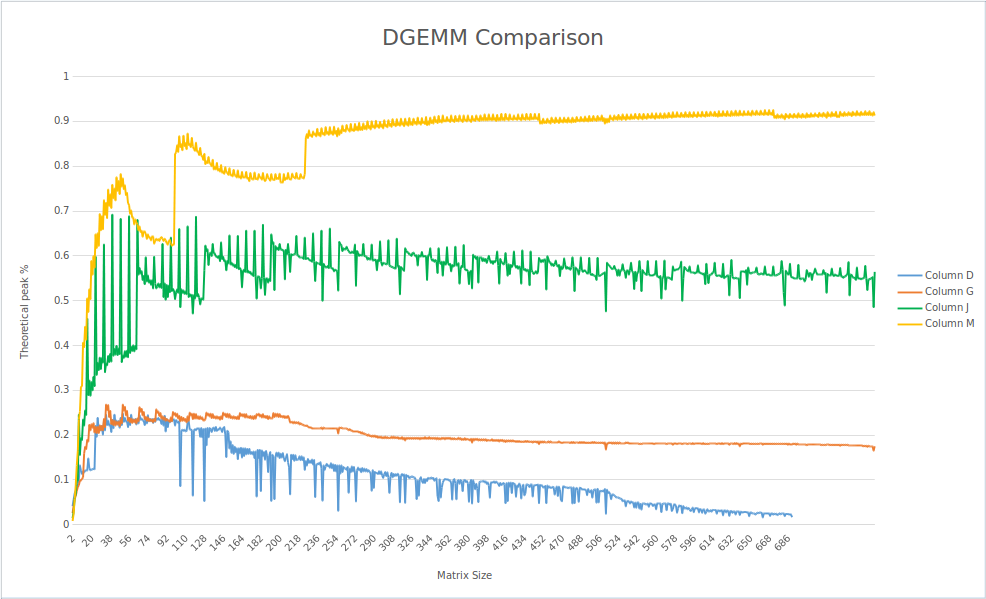
\includegraphics[width=0.9\linewidth]{comparison-graph-percentage.png}
  \caption{Comparing different algorithms in max theoretical percentage. Assuming Hopper has 8.4 GFLOPS.}
  \centering
  \label{fig:sub1}
\end{figure}

The max theoretical performance has been calculated, assuming hopper has 8.4 GFLOPS, using the following formula:

\begin{align*}
\frac{\text{(Actual GFLOPS)}}{8.4} = \text{Performance in \%}
\end{align*}

\subsection{Odd Behaviours}
% The reason for any odd behavior (e.g., dips) in performance.
The graph for our implementation (represented as a green) shows a constant decrease as sizes grow, for then to jump back up and resume the decrease from there. This behaviour comes from fringe cases where fringe size is below 8, as the fringes grows more and more in size until reaching size 8, where they can be unrolled again. This this decrease is a direct result of fringe cases not being unrolled to the same extend as the rest of the calculations.

As the matrix sizes grow larger and larger, these fringe cases means less and less overall, and thus the decrease resulting from this shows less of an impact on the graph.

Another odd behaviour is the ``spikes'' for every second plot, this is a direct result of the number being odd, and therefore needing to be padded when used in SSE instructions. Again this impact falls as sizes grow, because the fringe cases has less and less impact as the matrix grows.

\subsection{Peak Performance}
% Explain how you determined the peak performace, and again, the y-axis should
% say percentage of peak performance.

\begin{figure}[H]
  \centering
  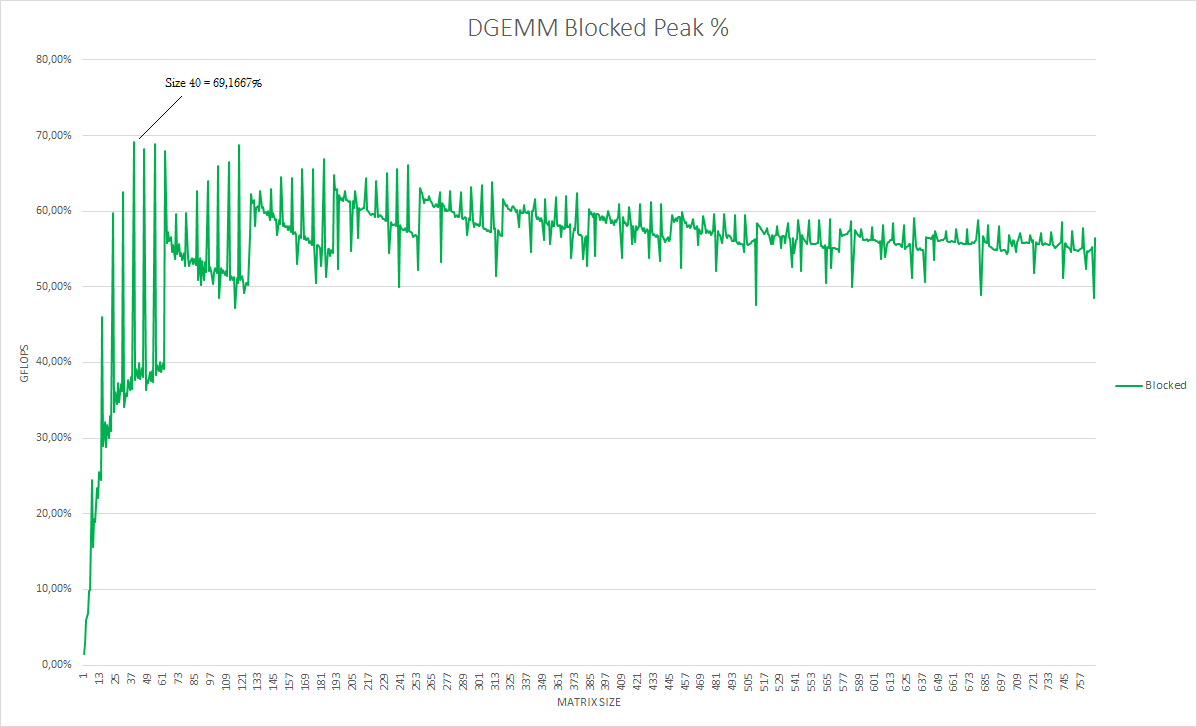
\includegraphics[width=0.9\linewidth]{peak-graph.png}
  \caption{Peak performance}
  \centering
  \label{fig:sub1}
\end{figure}

The average performance across sizes 2 to 769 is $55,235\%$, with a top peak-performance of $69.166\%$ with matrix size 40. The first have been calculated from finding the average runtime for all sizes and then dividing that number by 8,4. The peak has been found by taking the GFLOPS for size 40 and dividing that by 8.4.

\begin{align*}
\frac{5,81}{8,4} = 69.166%
\end{align*}

\section{IMADA Machines}
\subsection{Graphs}
% A figure fhat shows the performace similar than the figure above, but using
% all matrix sizes 2, 3, 4, ..., 769 for a single processor of another system of
% your choice (using the same kernel).

Below is a graph like the previous, but instead run on the Imada terminal room. When running these tests on the imada terminal room, we are working on an shared environment and thus performance may be affected by other users actions at the time of running. A single context-switch could cause the cache to flush all relevant data to memory and would then have to be loaded back in as the process resumes.

Likewise is it easy to see that the BLAS library is not nearly as fine-tuned in these machines as what we saw on Hopper.

\begin{figure}[H]
  \centering
  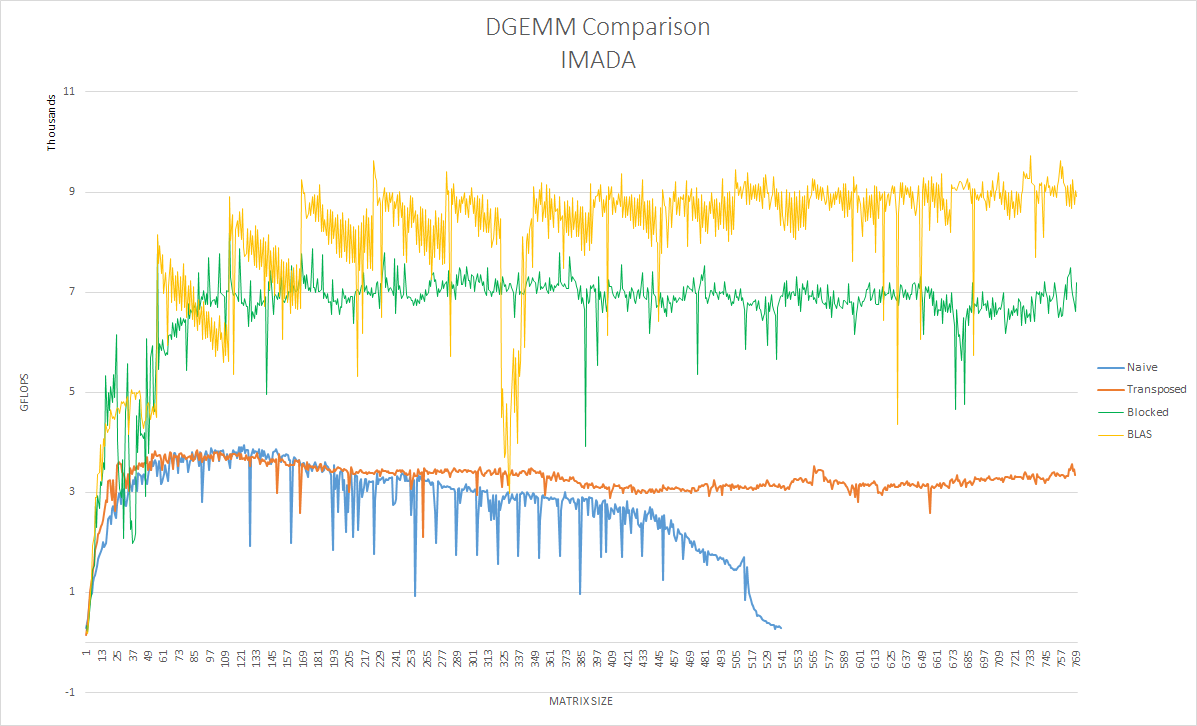
\includegraphics[width=0.9\linewidth]{comparison-graph-imada.png}
  \caption{Comparing different algorithms with our implementation. The Blocked is the performance we arrived at.}
  \centering
  \label{fig:sub1}
\end{figure}

It should be noted all these are run when using SSH, thus there is a decreased performance compared to logging directly in to a machine. % Dont know why but Rolf stated this.

\chapter{Conclusion}
% A short recap of what we achieved and the results.
An effective algorithm was implemented following idea mentioned from the goto article. Using these ideas and tweaking we managed an average of around 55\% of theoretical max performance, peaking into almost 70\%. 

We beat the BLAS implementation a couple of times for smaller matrix sizes, although for such small sizes the performance is not nearly as critical.


%-----------------------------------------------------------------
%						     APPENDIX
%-----------------------------------------------------------------
%\newpage
%\newgeometry{left=2.5cm,right=2.5cm}
%\chapter{Appendix}
%\section{Source code}

\end{document}
